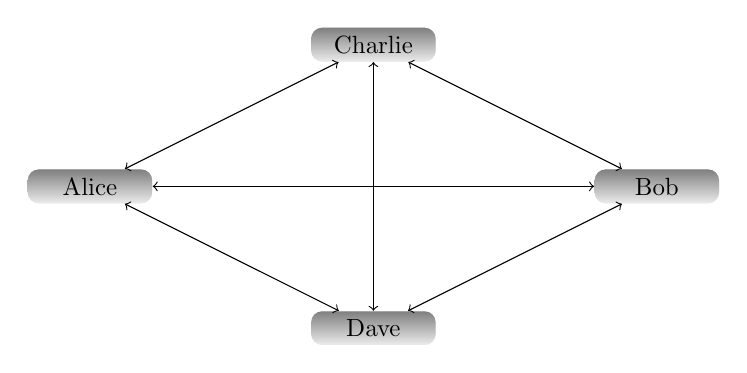
\begin{tikzpicture}[scale=.9,transform shape]
  \tikzstyle{every node} = [rectangle, rounded corners, fill=gray!20, bottom color=gray!15, minimum width=50pt]

  \onslide<+-> {
    \node (a) at (180: 4) {Alice};
    \node (b) at +(0: 4) {Bob};
  }

  \onslide<+-> {
    \draw [<->] (a) -- (b);
  }

  \onslide<+->{
    \node (c) at +(90: 2) {Charlie};
  }

  \onslide<+->{
    \draw [<->] (a) -- (c);
  }

  \onslide<+->{
    \draw [<->] (b) -- (c);
  }

  \onslide<+->{
    \node (d) at +(270: 2) {Dave};
  }

  \onslide<+->{
    \foreach \from/\to in {a/d, b/d, c/d}
      \draw [<->] (\from) -- (\to);
  }
\end{tikzpicture}
